\documentclass{article}
\usepackage[paperwidth=7.16in,paperheight=5.25in,margin=0.12in]{geometry}
\usepackage{amsmath}
\usepackage{amssymb}
\usepackage{tikz}
\usetikzlibrary{arrows.meta,positioning,calc,fit}
\pagestyle{empty}
\setlength{\parindent}{0pt}

\definecolor{prepblue}{RGB}{229,239,248}
\definecolor{prepblueedge}{RGB}{62,102,137}
\definecolor{alignviolet}{RGB}{239,234,247}
\definecolor{alignvioletedge}{RGB}{102,80,132}
\definecolor{complexgreen}{RGB}{231,243,235}
\definecolor{complexgreenedge}{RGB}{65,119,79}
\definecolor{baselinegray}{RGB}{242,242,242}
\definecolor{baselineedge}{RGB}{92,92,92}

\begin{document}
\centering
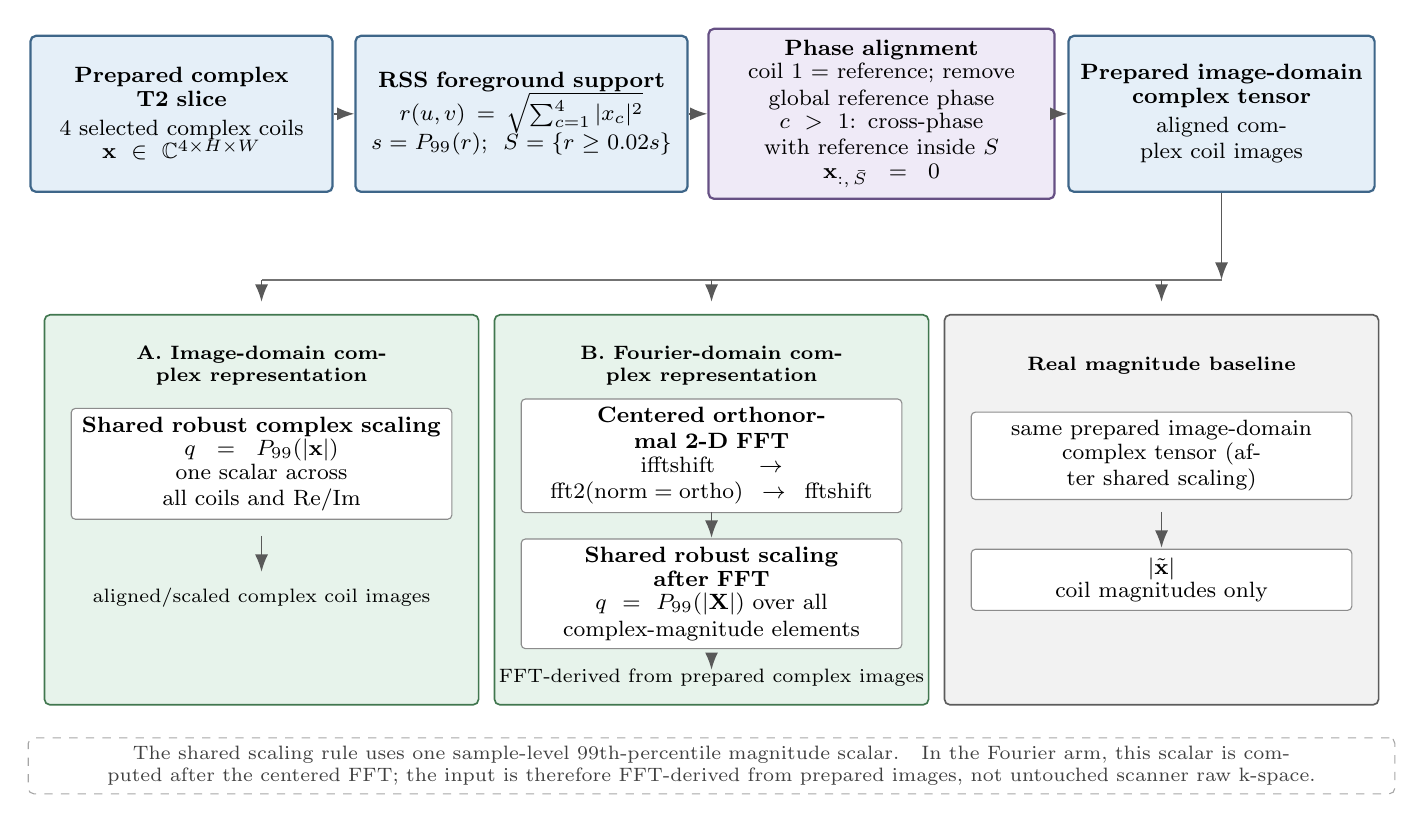
\begin{tikzpicture}[
  x=1in,y=1in,
  font=\footnotesize,
  >=Latex,
  arrow/.style={-{Latex[length=2.2mm]},semithick,draw=black!65},
  mainbox/.style={draw=black!65,rounded corners=2pt,thick,align=center,
    inner sep=4pt,text width=1.40in,minimum height=0.78in},
  supportbox/.style={mainbox,fill=prepblue,draw=prepblueedge,text width=1.55in},
  alignbox/.style={mainbox,fill=alignviolet,draw=alignvioletedge,text width=1.62in},
  tensorbox/.style={mainbox,fill=prepblue,draw=prepblueedge,text width=1.42in},
  lanebox/.style={draw=black!55,rounded corners=2pt,semithick,align=center,
    inner sep=4pt,text width=2.06in,minimum height=1.95in},
  rulebox/.style={draw=black!45,rounded corners=1.5pt,fill=white,
    inner sep=3pt,align=center,text width=1.82in},
  label/.style={font=\scriptsize,align=center,text=black!75},
  small/.style={font=\scriptsize,align=center},
  mathsmall/.style={font=\scriptsize,align=center}
]

% Main preprocessing path.
\node[mainbox,fill=prepblue,draw=prepblueedge] (input) at (-2.65,0.68) {\textbf{Prepared complex}\\[-1pt]\textbf{T2 slice}\\[1pt]
  4 selected complex coils\\[-1pt]
  $\mathbf{x}\in\mathbb{C}^{4\times H\times W}$};

\node[supportbox] (support) at (-0.95,0.68) {\textbf{RSS foreground support}\\[-1pt]
  $r(u,v)=\sqrt{\sum_{c=1}^{4}|x_c|^2}$\\[-1pt]
  $s=P_{99}(r)$; $\ S=\{r\ge 0.02s\}$};

\node[alignbox] (align) at (0.85,0.68) {\textbf{Phase alignment}\\[-1pt]
  coil 1 = reference; remove global reference phase\\[-1pt]
  $c>1$: cross-phase with reference inside $S$\\[-1pt]
  $\mathbf{x}_{:,\,\bar S}=0$};

\node[tensorbox] (tensor) at (2.55,0.68) {\textbf{Prepared image-domain}\\[-1pt]
  \textbf{complex tensor}\\[1pt]
  aligned complex coil images};

\draw[arrow] (input.east) -- (support.west);
\draw[arrow] (support.east) -- (align.west);
\draw[arrow] (align.east) -- (tensor.west);

% One visible fork, with the exact domain-specific order shown inside each lane.
\coordinate (fork) at (2.55,-0.15);
\draw[arrow] (tensor.south) -- (fork);
\draw[black!55,semithick] (fork) -- (-2.25,-0.15);
\draw[black!55,semithick] (fork) -- (2.25,-0.15);
\draw[arrow] (-2.25,-0.15) -- (-2.25,-0.26);
\draw[arrow] (0,-0.15) -- (0,-0.26);
\draw[arrow] (2.25,-0.15) -- (2.25,-0.26);

% Image-domain complex representation.
\node[lanebox,fill=complexgreen,draw=complexgreenedge] (imageLane) at (-2.25,-1.30) {};
\node[font=\scriptsize\bfseries,align=center,text width=2.0in] at (-2.25,-0.58)
  {A. Image-domain complex representation};
\node[rulebox] at (-2.25,-1.07) {\textbf{Shared robust complex scaling}\\[-1pt]
  $q=P_{99}(|\mathbf{x}|)$\\[-1pt]
  one scalar across all coils and Re/Im};
\node[small] at (-2.25,-1.74) {aligned/scaled complex coil images};
\draw[arrow] (-2.25,-1.43) -- (-2.25,-1.61);

% Fourier-domain complex representation.
\node[lanebox,fill=complexgreen,draw=complexgreenedge] (fourierLane) at (0,-1.30) {};
\node[font=\scriptsize\bfseries,align=center,text width=2.0in] at (0,-0.58)
  {B. Fourier-domain complex representation};
\node[rulebox] at (0,-1.03) {\textbf{Centered orthonormal 2-D FFT}\\[-1pt]
  $\mathrm{ifftshift}\;\to\;\mathrm{fft2}(\mathrm{norm=ortho})\;\to\;\mathrm{fftshift}$};
\node[rulebox] at (0,-1.72) {\textbf{Shared robust scaling}\\[-1pt]\textbf{after FFT}\\[-1pt]
  $q=P_{99}(|\mathbf{X}|)$ over all complex-magnitude elements};
\node[small] at (0,-2.14) {FFT-derived from prepared complex images};
\draw[arrow] (0,-1.31) -- (0,-1.44);
\draw[arrow] (0,-2.06) -- (0,-2.10);

% Real magnitude baseline.
\node[lanebox,fill=baselinegray,draw=baselineedge] (realLane) at (2.25,-1.30) {};
\node[font=\scriptsize\bfseries,align=center,text width=2.0in] at (2.25,-0.58)
  {Real magnitude baseline};
\node[rulebox] at (2.25,-1.03) {same prepared image-domain\\[-1pt]
  complex tensor (after shared scaling)};
\node[rulebox] at (2.25,-1.65) {$\displaystyle |\tilde{\mathbf{x}}|$\\[-1pt]
  coil magnitudes only};
\draw[arrow] (2.25,-1.31) -- (2.25,-1.49);

% Explicit implementation note: it prevents the Fourier arm from reading as raw k-space.
\node[draw=black!35,dashed,rounded corners=2pt,inner sep=3pt,align=center,
  font=\scriptsize,text=black!75,text width=6.75in] at (0,-2.58)
  {The shared scaling rule uses one sample-level 99th-percentile magnitude scalar.\quad
   In the Fourier arm, this scalar is computed after the centered FFT; the input is therefore FFT-derived from prepared images, not untouched scanner raw k-space.};
\end{tikzpicture}

\vspace{0.07in}
\begin{minipage}{6.86in}
\scriptsize
\textbf{Figure 2.} Preprocessing and representation pipeline used for the factorial study. Four prepared complex coil images are used to estimate an RSS foreground support, align global inter-coil phase offsets, and apply a shared sample-level robust magnitude scale within each representation. Complex models receive either the aligned image-domain tensor or its centered orthonormal FFT, while the real baseline receives the corresponding coil magnitudes.
\end{minipage}
\end{document}
